% This file was created by tikzplotlib v0.8.2.
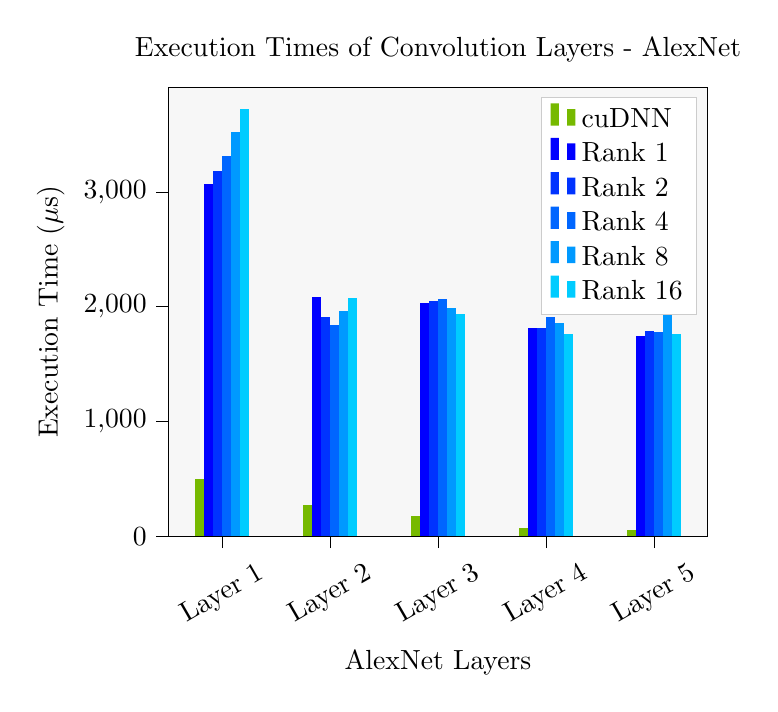
\begin{tikzpicture}

\definecolor{color0}{rgb}{0.462745098,0.7254901961,0}
\definecolor{color1}{rgb}{0,0.2,1}
\definecolor{color2}{rgb}{0,0.4,1}
\definecolor{color3}{rgb}{0,0.6,1}
\definecolor{color4}{rgb}{0,0.8,1}

\begin{axis}[
axis background/.style={fill=white!97.0!black},
legend cell align={left},
legend style={draw=white!80.0!black},
tick align=outside,
tick pos=left,
title={Execution Times of Convolution Layers - AlexNet},
x grid style={white!69.01960784313725!black},
xlabel={AlexNet Layers},
xmin=-0.5, xmax=4.5,
xtick style={color=black},
xtick={0,1,2,3,4},
xticklabel style = {rotate=30.0},
xticklabels={Layer 1,Layer 2,Layer 3,Layer 4,Layer 5},
y grid style={white!69.01960784313725!black},
ylabel={Execution Time (\(\displaystyle \mu\)s)},
ymin=0, ymax=3906,
ytick style={color=black}
]
\draw[fill=color0,draw opacity=0] (axis cs:-0.25,0) rectangle (axis cs:-0.166666666666667,499.412);
\addlegendimage{ybar,ybar legend,fill=color0,draw opacity=0};
\addlegendentry{ cuDNN}

\draw[fill=color0,draw opacity=0] (axis cs:0.75,0) rectangle (axis cs:0.833333333333333,270.704);
\draw[fill=color0,draw opacity=0] (axis cs:1.75,0) rectangle (axis cs:1.83333333333333,177.415);
\draw[fill=color0,draw opacity=0] (axis cs:2.75,0) rectangle (axis cs:2.83333333333333,71.3287);
\draw[fill=color0,draw opacity=0] (axis cs:3.75,0) rectangle (axis cs:3.83333333333333,52.1001);
\draw[fill=blue,draw opacity=0] (axis cs:-0.166666666666667,0) rectangle (axis cs:-0.0833333333333333,3069.5);
\addlegendimage{ybar,ybar legend,fill=blue,draw opacity=0};
\addlegendentry{ Rank 1}

\draw[fill=blue,draw opacity=0] (axis cs:0.833333333333333,0) rectangle (axis cs:0.916666666666667,2079.7);
\draw[fill=blue,draw opacity=0] (axis cs:1.83333333333333,0) rectangle (axis cs:1.91666666666667,2033.9);
\draw[fill=blue,draw opacity=0] (axis cs:2.83333333333333,0) rectangle (axis cs:2.91666666666667,1810);
\draw[fill=blue,draw opacity=0] (axis cs:3.83333333333333,0) rectangle (axis cs:3.91666666666667,1741.4);
\draw[fill=color1,draw opacity=0] (axis cs:-0.0833333333333333,0) rectangle (axis cs:-1.38777878078145e-17,3178.9);
\addlegendimage{ybar,ybar legend,fill=color1,draw opacity=0};
\addlegendentry{ Rank 2}

\draw[fill=color1,draw opacity=0] (axis cs:0.916666666666667,0) rectangle (axis cs:1,1911);
\draw[fill=color1,draw opacity=0] (axis cs:1.91666666666667,0) rectangle (axis cs:2,2047.5);
\draw[fill=color1,draw opacity=0] (axis cs:2.91666666666667,0) rectangle (axis cs:3,1812.5);
\draw[fill=color1,draw opacity=0] (axis cs:3.91666666666667,0) rectangle (axis cs:4,1790.6);
\draw[fill=color2,draw opacity=0] (axis cs:-3.46944695195361e-17,0) rectangle (axis cs:0.0833333333333333,3308.4);
\addlegendimage{ybar,ybar legend,fill=color2,draw opacity=0};
\addlegendentry{ Rank 4}

\draw[fill=color2,draw opacity=0] (axis cs:1,0) rectangle (axis cs:1.08333333333333,1838);
\draw[fill=color2,draw opacity=0] (axis cs:2,0) rectangle (axis cs:2.08333333333333,2066.2);
\draw[fill=color2,draw opacity=0] (axis cs:3,0) rectangle (axis cs:3.08333333333333,1907.5);
\draw[fill=color2,draw opacity=0] (axis cs:4,0) rectangle (axis cs:4.08333333333333,1779.8);
\draw[fill=color3,draw opacity=0] (axis cs:0.0833333333333333,0) rectangle (axis cs:0.166666666666667,3519.5);
\addlegendimage{ybar,ybar legend,fill=color3,draw opacity=0};
\addlegendentry{ Rank 8}

\draw[fill=color3,draw opacity=0] (axis cs:1.08333333333333,0) rectangle (axis cs:1.16666666666667,1961.8);
\draw[fill=color3,draw opacity=0] (axis cs:2.08333333333333,0) rectangle (axis cs:2.16666666666667,1985);
\draw[fill=color3,draw opacity=0] (axis cs:3.08333333333333,0) rectangle (axis cs:3.16666666666667,1860.3);
\draw[fill=color3,draw opacity=0] (axis cs:4.08333333333333,0) rectangle (axis cs:4.16666666666667,2399.3);
\draw[fill=color4,draw opacity=0] (axis cs:0.166666666666667,0) rectangle (axis cs:0.25,3720);
\addlegendimage{ybar,ybar legend,fill=color4,draw opacity=0};
\addlegendentry{ Rank 16}

\draw[fill=color4,draw opacity=0] (axis cs:1.16666666666667,0) rectangle (axis cs:1.25,2073.7);
\draw[fill=color4,draw opacity=0] (axis cs:2.16666666666667,0) rectangle (axis cs:2.25,1936.4);
\draw[fill=color4,draw opacity=0] (axis cs:3.16666666666667,0) rectangle (axis cs:3.25,1759.7);
\draw[fill=color4,draw opacity=0] (axis cs:4.16666666666667,0) rectangle (axis cs:4.25,1761.5);
\end{axis}

\end{tikzpicture}